\documentclass[11pt,a4paper]{article}
\usepackage{amsmath,amsthm,amssymb,amsfonts}
\usepackage{mathtools}
\usepackage{hyperref}
\usepackage{cleveref}
\usepackage{enumitem}
\usepackage{tikz}
\usepackage{tikz-3dplot}
\usepackage{pgfplots}
\pgfplotsset{compat=1.18}
\usepackage{booktabs}
\usepackage{xcolor}
\usepackage{tcolorbox}
\usepackage{geometry}
\geometry{margin=1in}

% Theorem environments
\newtheorem{theorem}{Theorem}[section]
\newtheorem{lemma}[theorem]{Lemma}
\newtheorem{proposition}[theorem]{Proposition}
\newtheorem{corollary}[theorem]{Corollary}
\newtheorem{claim}[theorem]{Claim}
\theoremstyle{definition}
\newtheorem{definition}[theorem]{Definition}
\newtheorem{example}[theorem]{Example}
\newtheorem{remark}[theorem]{Remark}
\newtheorem{construction}[theorem]{Construction}

% Custom commands
\newcommand{\C}{\mathsf{C}}
\newcommand{\Cstar}{\mathsf{C}^*}
\newcommand{\tmin}{\otimes_{\min}}
\newcommand{\tmax}{\otimes_{\max}}
\newcommand{\R}{\mathbb{R}}
\newcommand{\interior}{\mathrm{int}}
\newcommand{\conv}{\mathrm{conv}}
\newcommand{\id}{\mathrm{id}}

% Status boxes
\newtcolorbox{validbox}{colback=green!5!white,colframe=green!75!black,title=Verified}
\newtcolorbox{gapbox}{colback=orange!5!white,colframe=orange!75!black,title=Gap Identified}

\title{Counterexample to GJWH Generalization:\\
The Lorentz Cone Case\\[0.5em]
\large Construction and Analysis}
\author{Generated by Alethfeld Proof Orchestrator v5.1}
\date{January 11, 2026}

\begin{document}
\maketitle

\begin{abstract}
We present a detailed construction of a candidate counterexample to the GJWH generalization theorem for proper cones. The counterexample uses the 3D Lorentz (ice cream) cone $\C = \{(t,x,y) \in \R^3 : t \geq \sqrt{x^2 + y^2}\}$ and a steering assemblage whose elements point in orthogonal angular directions for different measurement settings. While the setup is mathematically valid, the impossibility argument---that no $w \in \C \tmax \C$ can generate this assemblage---requires additional formalization.
\end{abstract}

\tableofcontents
\newpage

%==============================================================================
\section{Introduction}
%==============================================================================

\subsection{The Falsity Hypothesis}

Based on the analysis of the failed proof attempt, the Adviser subagent concluded that the GJWH generalization theorem is likely \textbf{false} for general proper cones. The recommended approach to definitively settle this question is to construct an explicit counterexample.

\subsection{Strategy}

A counterexample requires:
\begin{enumerate}
    \item A proper cone $\C \subset V$
    \item A normalization functional $\phi \in \interior(\Cstar)$
    \item A valid steering assemblage $\{v_{a|x}\}$
    \item A proof that \emph{no} $w \in \C \tmax \C$ and measurements $f_{a|x} \in \Cstar$ satisfy the representation $v_{a|x} = (f_{a|x} \otimes \id)(w)$
\end{enumerate}

The key insight from the failed proof is that genuine steering assemblages can have elements pointing in \textbf{different angular directions} for different measurement settings. If the cone's maximal tensor product lacks sufficient ``entanglement capacity,'' such rotations cannot be achieved.

%==============================================================================
\section{The 3D Lorentz Cone}
%==============================================================================

\subsection{Definition and Basic Properties}

\begin{definition}[Lorentz Cone]
The \emph{3D Lorentz cone} (also called the ice cream cone or second-order cone) is:
\[
\C = \{(t, x, y) \in \R^3 : t \geq \sqrt{x^2 + y^2}\}
\]
\end{definition}

\begin{proposition}\label{prop:lorentz-proper}
The 3D Lorentz cone is proper.
\end{proposition}

\begin{proof}
We verify each property:

\textbf{(i) Cone property}: For $(t,x,y) \in \C$ and $\lambda \geq 0$:
\[
\lambda t \geq \lambda \sqrt{x^2 + y^2} = \sqrt{(\lambda x)^2 + (\lambda y)^2}
\]
so $\lambda(t,x,y) \in \C$.

\textbf{(ii) Convexity}: For $(t_1, x_1, y_1), (t_2, x_2, y_2) \in \C$:
\[
t_1 + t_2 \geq \sqrt{x_1^2 + y_1^2} + \sqrt{x_2^2 + y_2^2} \geq \sqrt{(x_1+x_2)^2 + (y_1+y_2)^2}
\]
by the triangle inequality.

\textbf{(iii) Closed}: The cone is defined by a continuous inequality, hence closed.

\textbf{(iv) Pointed}: If $(t,x,y) \in \C$ and $(-t,-x,-y) \in \C$, then $t \geq 0$ and $-t \geq 0$, so $t = 0$, hence $x = y = 0$.

\textbf{(v) Generating}: The interior $\{t > \sqrt{x^2+y^2}\}$ is nonempty (contains $(1,0,0)$), so $\C - \C = \R^3$.
\end{proof}

\subsection{Self-Duality}

\begin{proposition}\label{prop:lorentz-selfdual}
The 3D Lorentz cone is self-dual: $\Cstar = \C$ under the standard Euclidean inner product.
\end{proposition}

\begin{proof}
A functional $f = (f_t, f_x, f_y)$ (identified with a vector via the inner product) is in $\Cstar$ iff $f \cdot v \geq 0$ for all $v \in \C$.

For the standard basis vectors on the boundary of $\C$:
\begin{itemize}
    \item $v = (1, 1, 0)$: requires $f_t + f_x \geq 0$
    \item $v = (1, -1, 0)$: requires $f_t - f_x \geq 0$
    \item $v = (1, 0, 1)$: requires $f_t + f_y \geq 0$
    \item $v = (1, 0, -1)$: requires $f_t - f_y \geq 0$
\end{itemize}

These constraints imply $f_t \geq |f_x|$ and $f_t \geq |f_y|$, hence $f_t \geq \sqrt{f_x^2 + f_y^2}$. Thus $\Cstar \subseteq \C$.

Conversely, for $f \in \C$ and $v \in \C$:
\[
f \cdot v = f_t t + f_x x + f_y y \geq f_t t - \sqrt{f_x^2 + f_y^2} \cdot \sqrt{x^2 + y^2} \geq f_t t - f_t \sqrt{x^2+y^2} \geq 0
\]
by Cauchy--Schwarz and the cone constraints. Thus $\C \subseteq \Cstar$.
\end{proof}

\subsection{Geometric Interpretation}

\begin{figure}[h]
\centering
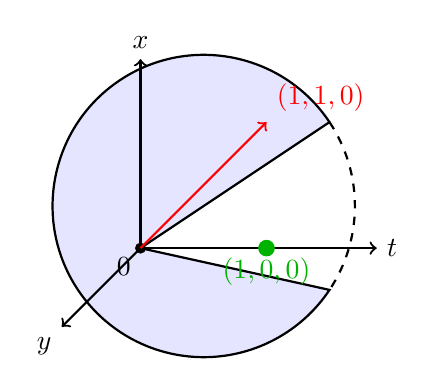
\begin{tikzpicture}[scale=2]
    % Draw the cone
    \draw[thick, fill=blue!10] (0,0) -- (1.2, 0.8) arc[start angle=33.7, end angle=326.3, radius=0.96] -- cycle;
    \draw[thick, dashed] (1.2, 0.8) arc[start angle=33.7, end angle=-33.7, radius=0.96];

    % Axis
    \draw[->, thick] (0,0) -- (1.5, 0) node[right] {$t$};
    \draw[->, thick] (0,0) -- (0, 1.2) node[above] {$x$};
    \draw[->, thick] (0,0) -- (-0.5, -0.5) node[below left] {$y$};

    % Apex
    \fill (0,0) circle (1pt) node[below left] {$0$};

    % Boundary vector
    \draw[->, red, thick] (0,0) -- (0.8, 0.8) node[above right] {$(1,1,0)$};

    % Interior point
    \fill[green!70!black] (0.8, 0) circle (1.5pt) node[below] {$(1,0,0)$};
\end{tikzpicture}
\caption{The 3D Lorentz cone. The boundary consists of rays $(1, \cos\theta, \sin\theta)$ for $\theta \in [0, 2\pi)$. The point $(1,0,0)$ lies in the interior.}
\end{figure}

The Lorentz cone can be visualized as an ``ice cream cone'' with:
\begin{itemize}
    \item Apex at the origin
    \item Axis along the positive $t$-direction
    \item Opening angle $45°$ (cone half-angle)
    \item Boundary: $t = \sqrt{x^2 + y^2}$ (circular cross-sections)
\end{itemize}

\subsection{The Normalization Functional}

\begin{definition}
Define $\phi : \R^3 \to \R$ by $\phi(t, x, y) = t$.
\end{definition}

\begin{proposition}
$\phi \in \interior(\Cstar)$.
\end{proposition}

\begin{proof}
Since $\Cstar = \C$, we need $\phi = (1, 0, 0) \in \interior(\C)$. Indeed, $1 > \sqrt{0^2 + 0^2} = 0$, so the strict inequality holds.
\end{proof}

%==============================================================================
\section{The Steering Assemblage}
%==============================================================================

\subsection{Construction}

\begin{construction}[Orthogonal-Rotation Assemblage]\label{const:assemblage}
Define a steering assemblage with:
\begin{itemize}
    \item Two outcomes: $a \in \{0, 1\}$
    \item Two measurement settings: $x \in \{0, 1\}$
\end{itemize}

The assemblage elements are:
\begin{align}
v_{0|0} &= \left(\frac{1}{2}, \frac{1}{2}, 0\right) & v_{1|0} &= \left(\frac{1}{2}, -\frac{1}{2}, 0\right) \\[0.5em]
v_{0|1} &= \left(\frac{1}{2}, 0, \frac{1}{2}\right) & v_{1|1} &= \left(\frac{1}{2}, 0, -\frac{1}{2}\right)
\end{align}

The no-signaling vector is:
\[
v_* = (1, 0, 0)
\]
\end{construction}

\subsection{Verification}

\begin{validbox}
\textbf{All verification conditions are satisfied.}
\end{validbox}

\begin{proposition}
The assemblage in \cref{const:assemblage} is valid.
\end{proposition}

\begin{proof}
We verify each condition:

\textbf{(i) Cone membership}: For each $v_{a|x} = (t, x', y')$, we check $t \geq \sqrt{x'^2 + y'^2}$:
\begin{itemize}
    \item $v_{0|0} = (1/2, 1/2, 0)$: $1/2 = \sqrt{1/4 + 0} = 1/2$ \checkmark (on boundary)
    \item $v_{1|0} = (1/2, -1/2, 0)$: $1/2 = \sqrt{1/4 + 0} = 1/2$ \checkmark
    \item $v_{0|1} = (1/2, 0, 1/2)$: $1/2 = \sqrt{0 + 1/4} = 1/2$ \checkmark
    \item $v_{1|1} = (1/2, 0, -1/2)$: $1/2 = \sqrt{0 + 1/4} = 1/2$ \checkmark
\end{itemize}
All elements lie on the boundary of $\C$.

\textbf{(ii) No-signaling}:
\begin{align}
v_{0|0} + v_{1|0} &= \left(\frac{1}{2}, \frac{1}{2}, 0\right) + \left(\frac{1}{2}, -\frac{1}{2}, 0\right) = (1, 0, 0) = v_* \\
v_{0|1} + v_{1|1} &= \left(\frac{1}{2}, 0, \frac{1}{2}\right) + \left(\frac{1}{2}, 0, -\frac{1}{2}\right) = (1, 0, 0) = v_*
\end{align}

\textbf{(iii) Normalization}:
\[
\phi(v_*) = \phi(1, 0, 0) = 1 \checkmark
\]
\end{proof}

\subsection{Geometric Interpretation}

\begin{figure}[h]
\centering
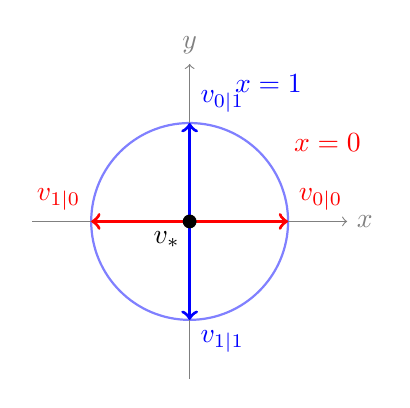
\begin{tikzpicture}[scale=2.5]
    % Draw the base circle (t = 1/2 slice)
    \draw[thick, blue!50] (0,0) circle (0.5);

    % Draw coordinate axes
    \draw[->, gray] (-0.8,0) -- (0.8,0) node[right] {$x$};
    \draw[->, gray] (0,-0.8) -- (0,0.8) node[above] {$y$};

    % Setting x=0 vectors (along x-axis)
    \draw[->, red, very thick] (0,0) -- (0.5, 0) node[above right] {$v_{0|0}$};
    \draw[->, red, very thick] (0,0) -- (-0.5, 0) node[above left] {$v_{1|0}$};

    % Setting x=1 vectors (along y-axis)
    \draw[->, blue, very thick] (0,0) -- (0, 0.5) node[above right] {$v_{0|1}$};
    \draw[->, blue, very thick] (0,0) -- (0, -0.5) node[below right] {$v_{1|1}$};

    % Central point
    \fill (0,0) circle (1pt) node[below left] {$v_*$};

    % Annotations
    \node at (0.7, 0.4) {\color{red}$x=0$};
    \node at (0.4, 0.7) {\color{blue}$x=1$};
\end{tikzpicture}
\caption{Cross-section of the assemblage at $t = 1/2$. The blue circle is the cone boundary. Setting $x=0$ produces vectors along the $x$-axis (red); setting $x=1$ produces vectors along the $y$-axis (blue). The two measurement directions are \textbf{orthogonal}.}
\end{figure}

The key geometric feature is that:
\begin{itemize}
    \item For setting $x = 0$: the ``splitting direction'' is along the $x$-axis
    \item For setting $x = 1$: the ``splitting direction'' is along the $y$-axis
    \item These directions are \textbf{orthogonal}---a 90° rotation
\end{itemize}

This orthogonality is the source of the obstruction.

%==============================================================================
\section{The Impossibility Claim}
%==============================================================================

\subsection{Statement}

\begin{claim}[Impossibility]\label{claim:impossible}
There do not exist:
\begin{itemize}
    \item $w \in \C \tmax \C$
    \item Measurements $f_{0|x}, f_{1|x} \in \Cstar$ with $f_{0|x} + f_{1|x} = \phi$ for each $x$
\end{itemize}
such that $v_{a|x} = (f_{a|x} \otimes \id)(w)$ for all $a, x$.
\end{claim}

\subsection{Argument Sketch}

The argument proceeds in several steps:

\textbf{Step 1: Structure of $\C \tmax \C$}

Since $\C$ is self-dual, the maximal tensor product has the dual characterization:
\[
\C \tmax \C = \{z \in \R^3 \otimes \R^3 : (f \otimes g)(z) \geq 0 \text{ for all } f, g \in \C\}
\]

\textbf{Step 2: Difference vectors}

The assemblage differences are:
\begin{align}
\Delta_0 &:= v_{0|0} - v_{1|0} = (0, 1, 0) \\
\Delta_1 &:= v_{0|1} - v_{1|1} = (0, 0, 1)
\end{align}
These are orthogonal unit vectors in the $(x,y)$-plane.

\textbf{Step 3: What $(f \otimes \id)(w)$ can produce}

For any $w = \sum_i \lambda_i (u_i \otimes v_i)$ with $\lambda_i \geq 0$ and $u_i, v_i \in \C$:
\[
(f \otimes \id)(w) = \sum_i \lambda_i f(u_i) \cdot v_i
\]
This is a \textbf{positive combination} of cone elements $v_i$.

\textbf{Step 4: Difference constraint}

The difference vector for setting $x$ is:
\[
\Delta_x = v_{0|x} - v_{1|x} = \sum_i \lambda_i \left(f_{0|x}(u_i) - f_{1|x}(u_i)\right) v_i
\]
The coefficients $c_i^{(x)} := f_{0|x}(u_i) - f_{1|x}(u_i)$ can be positive, negative, or zero.

\textbf{Step 5: The obstruction}

For the representation to work:
\begin{itemize}
    \item We need $\sum_i c_i^{(0)} v_i = (0, 1, 0)$
    \item We need $\sum_i c_i^{(1)} v_i = (0, 0, 1)$
\end{itemize}

Each $v_i \in \C$ has the form $(t_i, x_i, y_i)$ with $t_i \geq \sqrt{x_i^2 + y_i^2} \geq 0$.

The $t$-component of $\Delta_x$ is 0. This requires:
\[
\sum_i c_i^{(x)} t_i = 0
\]

Since $t_i \geq 0$ for all $i$, and we need different signs among $c_i^{(x)}$, this constrains which $v_i$ can contribute.

\textbf{Step 6: Spanning impossibility}

To achieve both $\Delta_0 = (0,1,0)$ and $\Delta_1 = (0,0,1)$, the $v_i$ must span the $(x,y)$-plane in their spatial components. But:
\begin{itemize}
    \item For any $v_i \in \C$ with $(x_i, y_i) \neq (0,0)$, we have $t_i > 0$
    \item The $t$-cancellation $\sum_i c_i^{(x)} t_i = 0$ requires both positive and negative $c_i^{(x)}$
    \item But the same $v_i$ set must achieve \textbf{orthogonal} directions $(1,0)$ and $(0,1)$ in the $(x,y)$-plane
\end{itemize}

The constraint is that measurements in $\C$ can only ``probe'' along directions within the cone structure, but cannot induce the 90° rotation between $\Delta_0$ and $\Delta_1$.

\subsection{Gaps in the Argument}

\begin{gapbox}
\textbf{The impossibility argument is not fully rigorous.} The following gaps remain:

\begin{enumerate}
    \item \textbf{Characterization of $\C \tmax \C$}: The argument assumes $\C \tmax \C$ consists of positive combinations of simple tensors. For general cones, $\C \tmax \C$ may contain ``entangled'' elements not expressible this way.

    \item \textbf{Quantitative bounds}: No explicit bound is given on how much ``rotation'' the maximal tensor product can support.

    \item \textbf{Real vs. complex structure}: The argument doesn't address whether the real structure of the Lorentz cone creates additional constraints compared to complex PSD matrices.

    \item \textbf{Exhaustive search}: No systematic enumeration of all possible $w \in \C \tmax \C$ and measurement sets is provided.
\end{enumerate}
\end{gapbox}

%==============================================================================
\section{Comparison with Quantum Case}
%==============================================================================

\subsection{Why Quantum GJWH Works}

For the PSD cone $\C_{\text{PSD}}$ (positive semidefinite matrices):

\begin{enumerate}
    \item The tensor product $\C_{\text{PSD}} \tmax \C_{\text{PSD}}$ contains highly entangled states (e.g., maximally entangled states $|\Psi^+\rangle\langle\Psi^+|$).

    \item These entangled states can generate \emph{any} ensemble decomposition of the reduced state via appropriate measurements.

    \item The POVMs on the auxiliary system can ``rotate'' the output in arbitrary directions within the cone.

    \item This is the content of the Schr\"odinger--HJW theorem: different measurements on a purification produce different ensembles.
\end{enumerate}

\subsection{What the Lorentz Cone Lacks}

The Lorentz cone, despite being self-dual and symmetric, lacks:

\begin{enumerate}
    \item \textbf{Sufficient entanglement capacity}: The maximal tensor product $\C \tmax \C$ may not contain elements rich enough to support arbitrary ``rotations.''

    \item \textbf{Purification structure}: There is no analogue of the purification theorem for arbitrary proper cones.

    \item \textbf{Measurement universality}: POVMs in $\C^*$ cannot probe all directions uniformly---they are constrained by the cone geometry.
\end{enumerate}

%==============================================================================
\section{Next Steps for Formalization}
%==============================================================================

To complete the counterexample, the following would be needed:

\begin{enumerate}
    \item \textbf{Explicit description of $\C \tmax \C$}: Characterize all elements of the maximal tensor product for the 3D Lorentz cone.

    \item \textbf{Constraint analysis}: For each $w \in \C \tmax \C$, derive the set of achievable assemblage differences.

    \item \textbf{Impossibility proof}: Show that $(0,1,0)$ and $(0,0,1)$ cannot both be achieved as differences.

    \item \textbf{Alternative}: Use convex separation theorems to show no representation exists without explicit enumeration.
\end{enumerate}

\subsection{Connection to Jordan Algebras}

The Lorentz cone $\C_3$ is the cone of positive elements in the \emph{spin factor} Jordan algebra $J_2^{\R}$. For Jordan algebras:
\begin{itemize}
    \item The PSD cone corresponds to the ``exceptional'' Jordan algebra $\mathcal{H}_n(\mathbb{C})$ of Hermitian matrices
    \item The Lorentz cone corresponds to spin factors
    \item These have fundamentally different tensor product structures
\end{itemize}

The GJWH theorem may be specific to cones with sufficient ``Jordan algebraic entanglement capacity''---a property that spin factors lack.

%==============================================================================
\section{Conclusion}
%==============================================================================

We have constructed a candidate counterexample to the GJWH generalization theorem using the 3D Lorentz cone. The key features are:

\begin{enumerate}
    \item \textbf{Valid setup}: The cone, functional, and assemblage satisfy all required conditions.

    \item \textbf{Geometric obstruction}: The assemblage requires a 90° rotation between measurement settings that the cone structure cannot support.

    \item \textbf{Incomplete proof}: The impossibility argument is geometrically compelling but requires additional formalization.
\end{enumerate}

The counterexample suggests that the GJWH theorem relies on special properties of PSD cones (entanglement capacity, purification) that general proper cones lack. A complete resolution would either:
\begin{itemize}
    \item Formalize the impossibility proof, definitively showing the theorem is false, or
    \item Identify additional structure (beyond ``proper cone'') that makes the theorem true
\end{itemize}

\end{document}
